\documentclass{article}
% \usepackage[spanish]{babel}
\usepackage[utf8]{inputenc}
\usepackage{graphicx}
\title{Ecuaciones en diferencias}
\author{Oconer}
\date{18 de septiembre de 2017}
\begin{document}
\maketitle

\section{Ecuaciones de primer grado}
\subsection{Ecuaciones lineales}
Una ecuación lineal en diferencias de primer orden tiene la forma $x_{n+1}=ax_n$
donde $a$ es una constante.

La fórmula para resolver ecuaciones lineales es:
\begin{equation}
\label{eq:2}
  x_n=a^nx_0
\end{equation}
por ejemplo, si iniciamos una inversión con 1000 pesos con un interes mensual del 1\%, obtenemos lo siguiente:

\begin{center}
  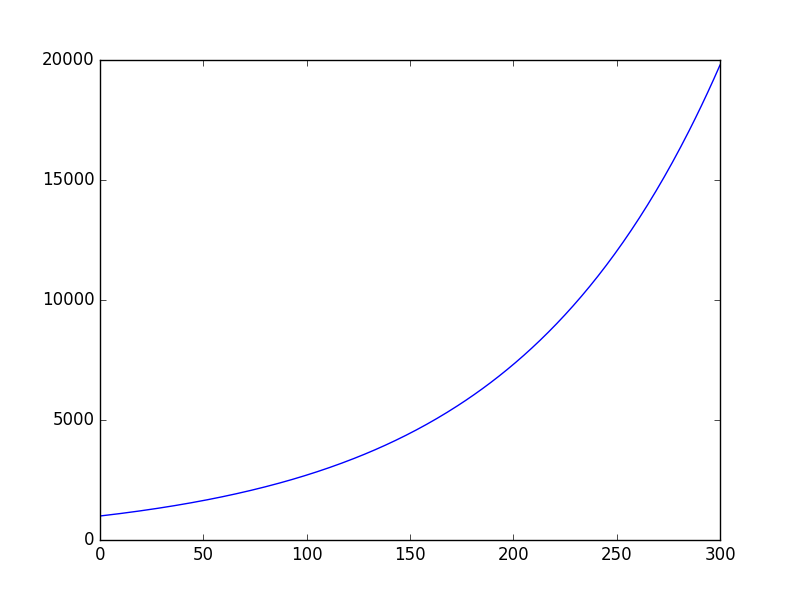
\includegraphics[width=8.5cm]{inversion.png}
\end{center}


\subsection{Ecuaciones afines}
Una ecuación afin en diferencias de primer grado tiene la forma $x_(n+1)=ax_n+b$
donde $a$ y $b$ son constantes.

\begin{equation}
 \label{eq:1}
  x_n=a^n(x_o-\alpha)+\alpha
\end{equation}
 donde $\alpha=\frac{b}{1-a}$.

 Para deducir esta formula usamos que
  $$\sum_{i=0}^{n-1}a^i=\frac{a^n-1}{a-i}$$

 \section{Ecuaciones de segundo grado}
 El método para resolver estas ecuaciones está inspirado en la fórmula \ref{eq:2}
 
\end{document}
